\documentclass[10pt]{article}

\linespread{1.5}
\usepackage{acmart}
\usepackage{libertine, graphicx}
\usepackage{natbib}
\usepackage{inconsolata}
\usepackage{hyperref}


\begin{document}
\title{Bandwidth and Latency Measurement on Inter-Process Communications}
\author{Kedar Bastakoti, Ruohui Wang}
\date{}

\maketitle

\begin{abstract}
    There are multiple ways to do inter-process communications(IPC). For example, pipe is often used to communicate between processes, whereas TCP and UDP can also be used to communicate both locally and remotely. Due to their differences in design, they tend to have different latencies and througputs. Experiments to show
\end{abstract}

\section{Clock Resolution}

To begin with, we need tools to measure the time.

The Linux operating system provides multiple system calls to measure the time, in different resolutions.

As per the POSIX manual\cite{posix_clock_gettime}, the function \texttt{gettimeofday} is obsolete so we chose \texttt{clock\_gettime} instead.

Also, the x86 CPU provides \texttt{rdtscp} instruction to give the CPU timestamp, in terms of .

The resolution is the smallest possible increase of the clock. In order to measure the resolution, we tried to create minimal possible differences between two time measurements. We create such difference by inserting an line of assembly \texttt{inc r12} into the code. And the result shows we are producing

However, along with \texttt{clock\_gettime}, function \texttt{clock\_getres} is provided for user to query the resolution of time. As we demonstrated later, it produces the same result as ours.
\section{System Calls}

Since we are measuring I/O performance, we cannot avoid doing a lot of system calls. System calls usually involve context switching, and trapping into the kernel. To get a better idea of how these system calls take up time. We measured some trivial system calls to see if the influence is actually trivial.

To measure the impact, we repeatedly make system calls that do least extra work. Here, we chose \texttt{getpid} and \texttt{getuid} as our syscalls. In addition, to avoid function returns that may take up time, we directly used the inline assembly to call the \texttt{syscall} instruction. And we return the minimum across all measurements to eliminate the effects of random events including page faults and preemptions.
\section{Pipe}
\section{TCP}
TCP uses sockets to communicate the between the hosts which is used across local or remote communication. TCP uses byte-ordered reliable communication mechanism which is widely supported across today's operating systems. In order to measure the latency and throughput of the TCP stream sockets, packet sizes of 4, 16, 64, 256, 1K, 4K, 16K, 64K, 256K, and 512K were considered.

We hypothesized that the latency will proportionally increase with the packet size, and the throughput will also increase as the packet sizes are increased. To get the most accurate representation of the results the test for each individual transfer unit was repeated 1 million times and the minimum number amongst those 1 million trials was considered to be the value closest to the real value.

One of the issues encountered while measuring TCP latency was that when using the read and write function calls of the Rust language on TCP stream, the functions were reading and writing random bytes of data which were different than the expected values. This caused discrepancies in the read and write sequence of the server and the client model. To remedy this problem, we switched to different function calls, read_all and write_all, which helped synchronize the flow of data between the client and the server.

%results



\section{UDP}
\section{Evaluation}
% Here should be the experimental setup, and results

We ran the experiments on the instructional machines, with Intel(R) Core(TM) i5-4570 CPU @ 3.20GHz, with 8GB RAM. The results are followed.

% lacking resolution & systemcall results

\begin{figure}[!ht]
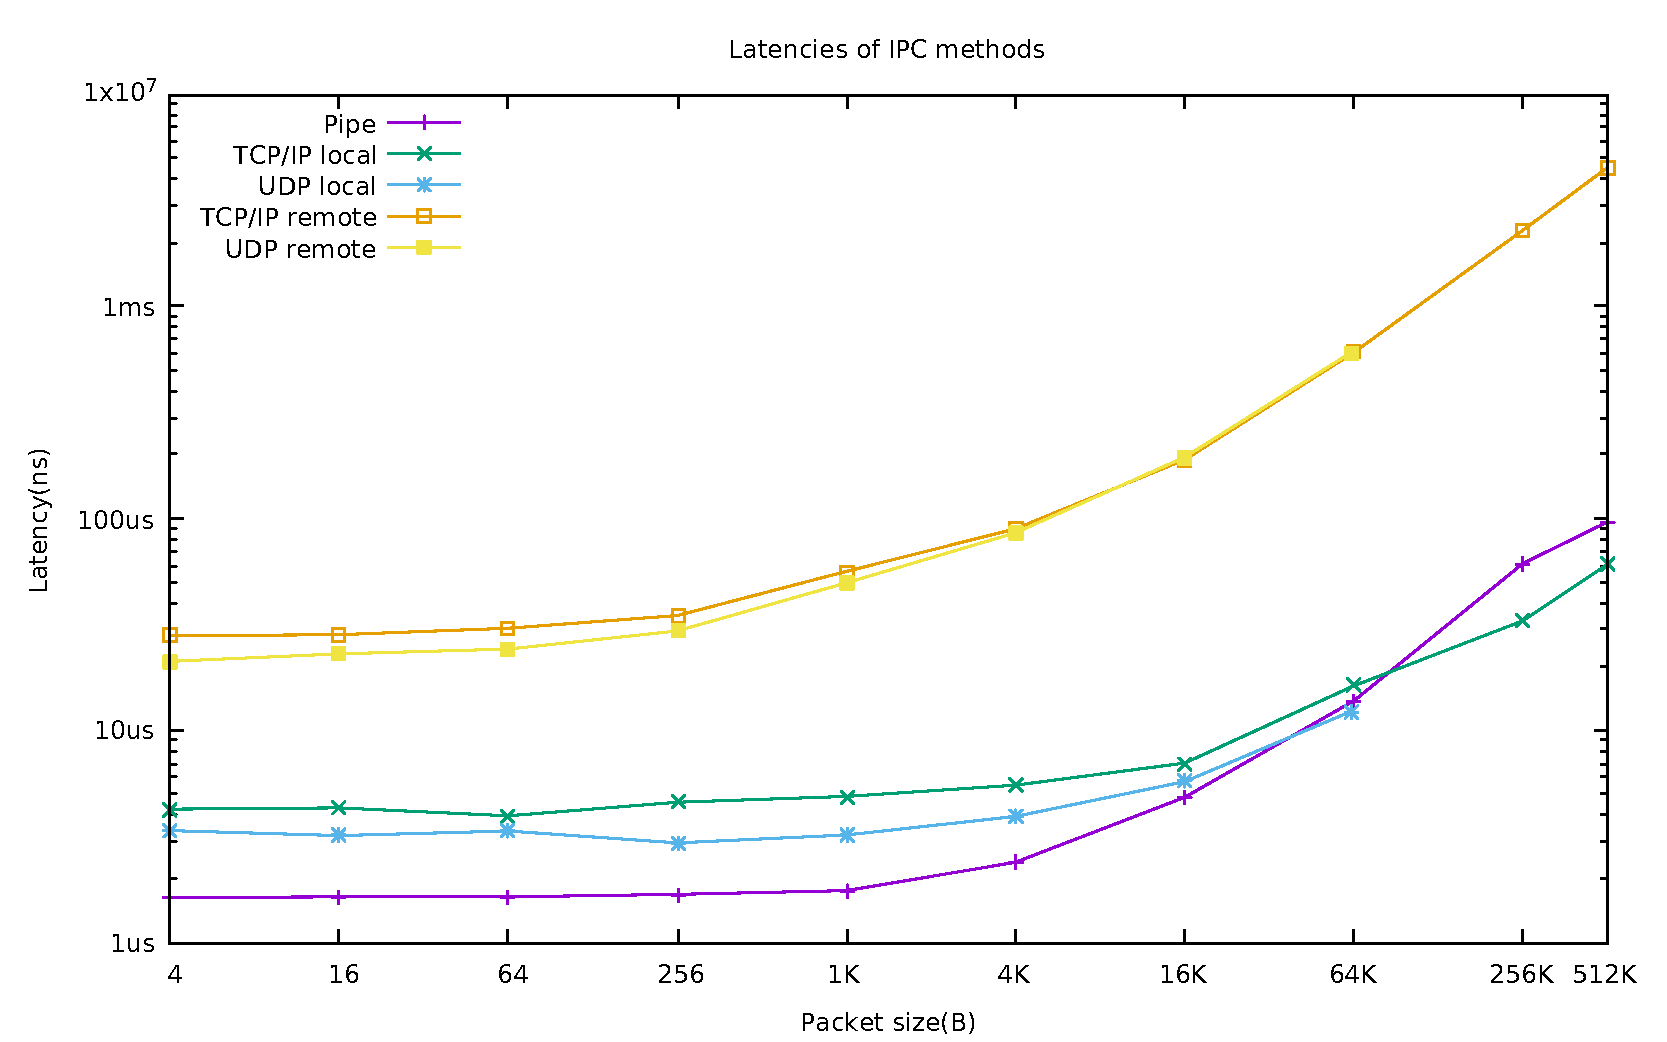
\includegraphics[width=.7\linewidth]{figures/latency}
\label{figure:latency}
\end{figure}

\begin{figure}[!ht]
    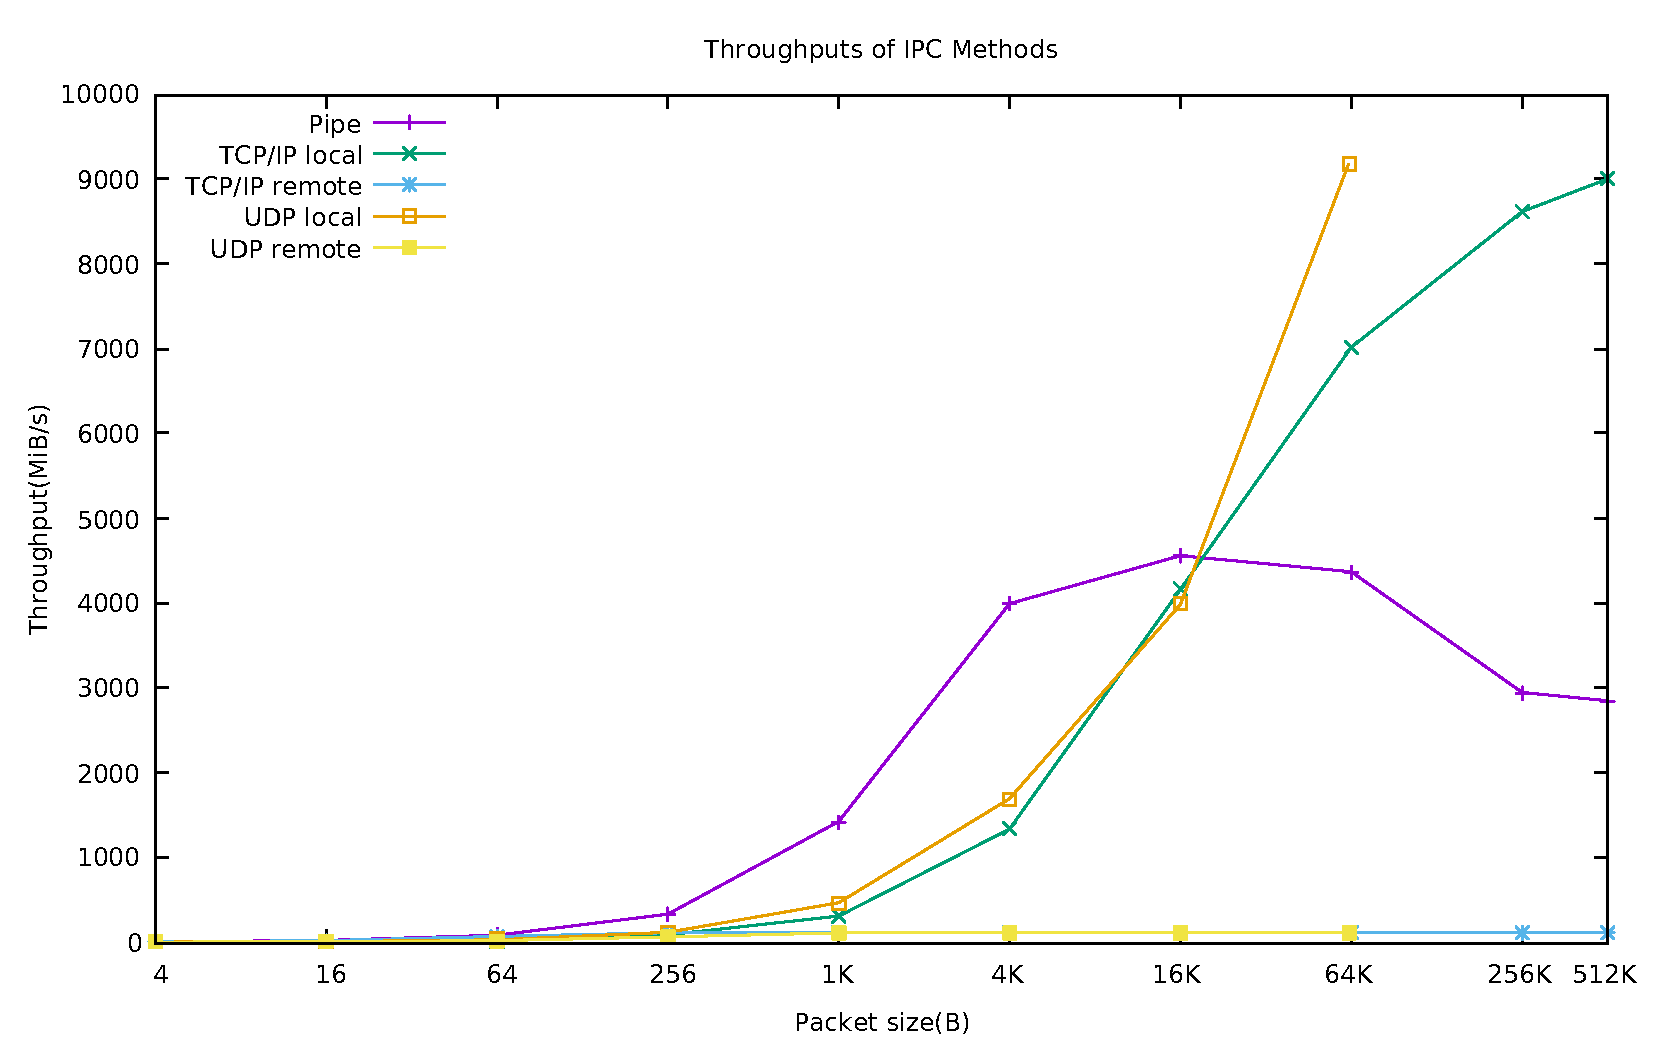
\includegraphics[width=.7\linewidth]{figures/throughput.pdf}
    \label{figure:throughput}
\end{figure}

\section{Conclusion}

\bibliographystyle{ACM-Reference-Format}
\bibliography{bibliography}
    
\end{document}